\chapter{Assessing the evolution of clouds and radiation in successive versions of a GCM: from CAM3 to CAM5}
\label{camamip}
\section{Introduction}
Climate models are continually updated as understanding of the climate system improves, new numerical techniques are more sophisticated physics parameterizations are developed, and computational resources are expanded to accommodate the increased complexity of the resulting models. In making changes from one model to the next, it is important to assess the impact of changes to the model on the simulated climate.

The relative performance of three recent versions of the NCAR CAM in terms of radiatively important cloud statistics is evaluated in this chapter. It is shown that many (but not all) measures of model cloud performance improve in successive versions of the model. The latest version of the model shows substantial improvement over the previous versions and over other models previously documented in the literature, owing largely to an improved and more realistic representation of subgrid-scale physics processes by way of a more sophisticated parameterization package.

\section{Model and experiment set-up}
This chapter extends the analysis of the previous chapter to versions 4 and 5 of the NCAR CAM. The CAM4 and CAM5 simulations cover a 10-year period from 2001-2010. This period differs from that done in the previous chapter for CAM3 and AM2, but Figure \ref{cldtot_obs_taylor} suggests that the affect of this differing averaging period should be inconsequential, and the model biases are shown to be much larger than any slight variation in climate in the differing periods of study.

The formulation of the different versions of the CAM provide a unique opportunity to study somewhat separately the effects of dynamics and parameterizations on the modeled cloud statistics. CAM3 and CAM4 are in many ways very similar models, sharing many subgrid-scale physics parameterizations. The major changes from CAM3 to CAM4 include a new finite volume default dynamical core, and changes to the parameterization of deep convection. CAM5 on the other hand is a very different model. CAM4 and CAM5 use the same dynamical core and deep convection parameterization, but CAM5 contains an otherwise completely updated, more physically consistent physics parameterization suite.

Although CAM3 and CAM4 appear to be very similar models, substantial and surprising differences in the representation of clouds between the two will be illustrated in the subsequent analysis. In an effort to better evaluate these differences, a CAM3 simulation with a finite volume dynamical core is added to the analysis.

\section{Results}
As noted previously, clouds are of primary importance in climate models because of their impact on the radiative budget. This is quantified by the cloud radiative effect. Biases in the shortwave and longwave cloud radiative effect between CAM4 and CAM5 and observations from CERES-EBAF are shown in Figures \ref{swcrebiases_camamip_map} and \ref{lwcrebiases_camamip_map}. As was seen for CAM3 and AM2 AMIP simulations, substantial compensating regional biases exist in both the shortwave and longwave cloud radiative effect in both CAM4 and CAM5 AMIP simulations. Substantial differences between CAM3 and CAM4 are readily apparent in Figures \ref{swcrebiases_camamip_map} and \ref{lwcrebiases_camamip_map}. The CAM4 simulation shows an overestimation of the magnitude of the shortwave cloud radiative effect throughout the tropics, with an underestimation in mid to high latitude regions. The CAM3 simulation shows regions of large underestimation of the magnitude of the shortwave cloud radiative effect in the tropics, especially in the ITCZ and in the tropical western Pacific. Biases in the longwave cloud effect are different in these same regions as well. Because these regions are known to be characterized by large overturning circulations and deep convection, these difference likely reflect the changes made in the deep convection parameterization. Other factors could also contribute to the differences, including differences in the dynamics or model-dependent tuning. Regional biases in the shortwave cloud radiative effect in CAM4 seem to share more similarities with CAM5 than with CAM3, as does the magnitude of the global mean bias. 
\begin{figure}
    \centering
    \includegraphics{../graphics/swcrebiases_camamip_map.pdf}
    \caption[Biases in shortwave cloud radiative effect in CAM3, CAM4, and CAM5 AMIP simulations compared with observations from CERES-EBAF.]{Biases in shortwave cloud radiative effect in CAM3, CAM4, and CAM5 AMIP simulations compared with observations from CERES-EBAF. Values in the titles of the individual plots indicate the area-weighted global mean bias between the model and observations.}
    \label{swcrebiases_camamip_map}
\end{figure}

\begin{figure}
    \centering
    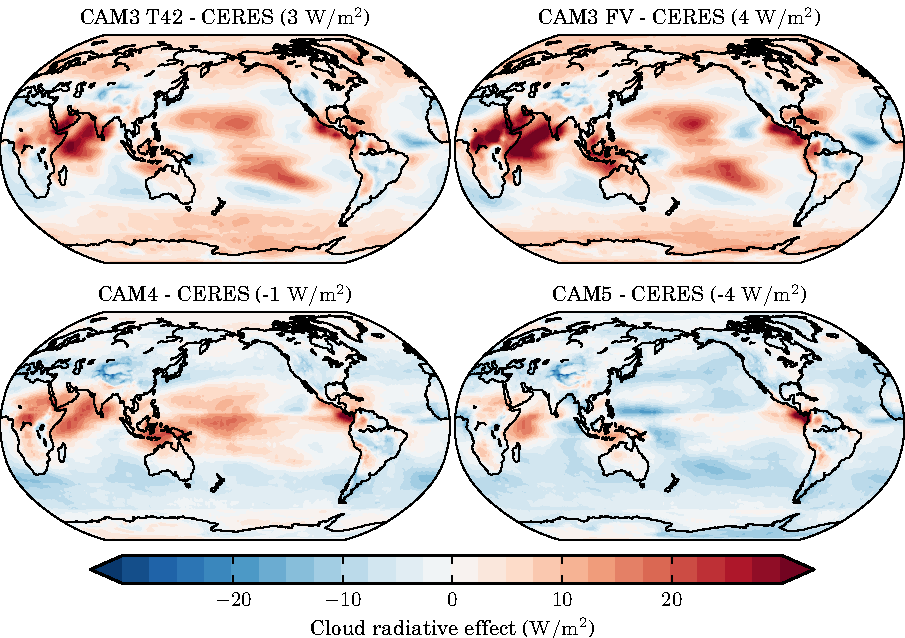
\includegraphics{../graphics/lwcrebiases_camamip_map.pdf}
    \caption[Biases in longwave cloud radiative effect in CAM4 and CAM5 AMIP simulations compared with observations from CERES-EBAF.]{Biases in longwave cloud radiative effect in CAM3, CAM4, and CAM5 AMIP simulations compared with observations from CERES-EBAF. Values in the titles of the individual plots indicate the area-weighted global mean bias between the model and observations.}
    \label{lwcrebiases_camamip_map}
\end{figure}

The agreement in the shortwave and longwave cloud radiative effect between all model simulations and observations is summarized in Figure \ref{cre_camamip_taylor}. This figure shows that the correlation improves in each successive version of CAM, although the spatial-temporal variability of the shortwave cloud radiative effect most closely matches the CERES-EBAF observations in the CAM4 simulation. The mean biases compared to the CERES-EBAF dataset are also lower in the CAM4 simulation than for the other model simulation shown here. All model simulations overestimate the magnitude of the shortwave cloud radiative effect (indicated by negative mean biases in each comparison in Figure \ref{swcrebiases_camamip_map}). Figure \ref{lwcrebiases_camamip_map} shows that the CAM3 simulations show an overestimation of the magnitude of the longwave cloud radiative effect, while the CAM4 and CAM5 simulations show an overall underestimation.

The correlation between the ERBE and CERES-EBAF datasets is much higher than that between any of the models and the CERES-EBAF dataset, giving confidence in conclusions drawn regarding the spatial-temporal correlation between model simulations and observations. The ratio of the variances and the relative ``biases'' in these fields between the ERBE dataset and the CERES-EBAF dataset are comparable with those seen in the comparisons between the model simulations and the CERES-EBAF dataset, giving less confidence in the robustness of conclusions drawn regarding these statistical quantities (though it should be noted that the ERBE dataset is only four years in length). The main conclusion from Figure \ref{cre_camamip_taylor}, is that the shortwave and longwave cloud radiative effect is better correlated with observations in space and time in CAM5 than in the two previous versions of CAM.
\begin{figure}
    \centering
    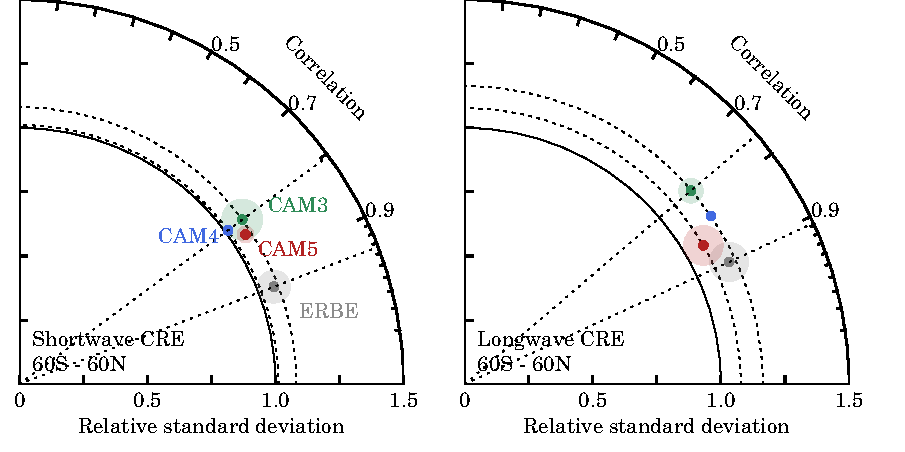
\includegraphics{../graphics/cre_camamip_taylor.pdf}
    \caption[Taylor diagrams comparing shortwave and longwave cloud radiative effect from CAM3, CAM4, and CAM5 AMIP simulations with observations from CERES-EBAF.]{Taylor diagrams comparing shortwave and longwave cloud radiative effect from CAM3, CAM4, and CAM5 AMIP simulations with observations from CERES-EBAF. Shortwave and longwave cloud radiative effect from the Earth Radiative Budget Experiment (ERBE) \citep{harrison_et_al_1990} are compared against the CERES-EBAF dataset as well.}
    \label{cre_camamip_taylor}
\end{figure}

Total, low, middle, and high-topped cloud amounts from ISCCP, MISR, and MODIS and their corresponding simulator diagnostics from CAM3, CAM4, and CAM5 AMIP simulations are shown in Figure \ref{cldtypes_camamip_bar}. As seen in the CAM3 and AM2 evaluation, total and low-topped cloud is underestimated in all models simulations. This is consistent with previous studies identifying underestimation of cloudiness in models \citep{zhang_et_al_2005}. Mid-topped cloud is underestimated in all model simulations except for in CAM5, which shows greatly reduced biases in ISCCP and MISR-simulated mid-topped cloud and a positive bias in MODIS-simulated mid-topped cloud. This result has been documented in \cite{kay_et_al_2011}, and shows that the long-standing negative bias in model-simulated, mid-topped cloud amount identified in \cite{zhang_et_al_2005} is reduced in CAM5, although differences in the sign of the bias when the MODIS comparison is added to the analysis are suggestive of uncertainty in these comparisons. High-topped cloud in CAM5 is shown here to be generally underestimated compared with the observations, while high-topped cloud is generally overestimated in the CAM3 simulations. Biases in ISCCP and MISR-simulated high-topped cloud are also negative in CAM4, although MODIS-simulated high-topped cloud is overestimated. 
\begin{figure}
    \centering
    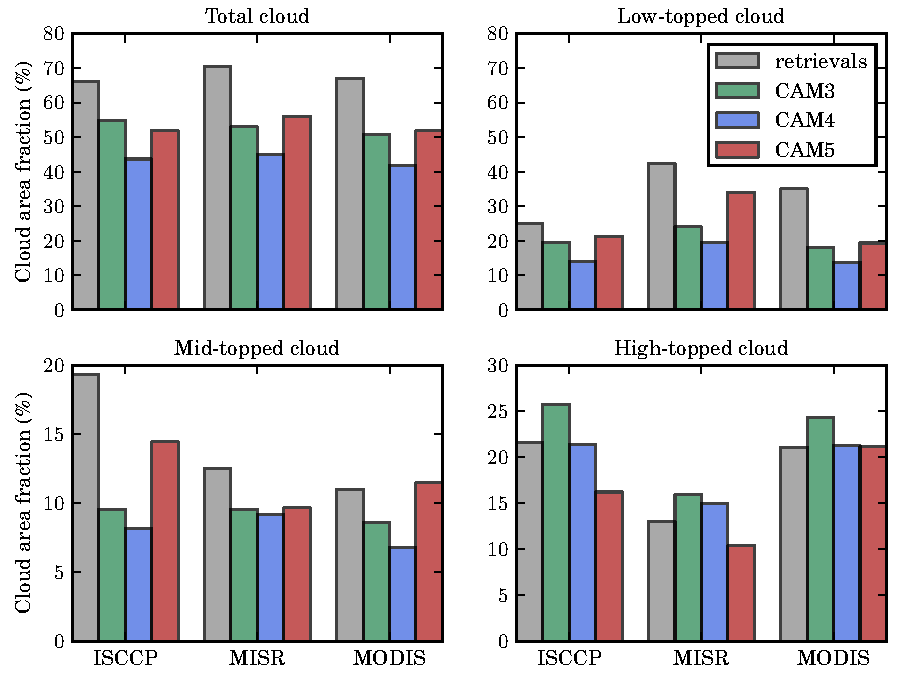
\includegraphics{../graphics/cldtypes_camamip_bar.pdf}
    \caption[Total, low-topped, mid-topped, and high-topped cloud amount from ISCCP, MISR, and MODIS and corresponding simulator diagnostics from CAM3, CAM4, and CAM5 AMIP simulations.]{Total, low-topped, mid-topped, and high-topped cloud amount from ISCCP, MISR, and MODIS and corresponding simulator diagnostics from CAM3, CAM4, and CAM5 AMIP simulations. MODIS cloud amounts are taken before clear-sky restoral.}
    \label{cldtypes_camamip_bar}
\end{figure}

Statistics for ISCCP, MISR, and MODIS-simulated total, low, mid, and high-topped clouds are compared with ISCCP, MISR, and MODIS observations in Figure \ref{cldtypes_camamip_taylor}. The different cloud types show at best moderate spatial-temporal correlation with observations, relative to the spatial-temporal correlation between the observations of total cloud amount shown in Figure \ref{cldtot_obs_taylor}. Nonetheless, CAM5 shows systematically better correlation with observations in almost every cloud type. Variance ratios between CAM5 and observed cloud types are also improved, indicating a spatial-temporal variability in CAM5 clouds that more closely matches the spatial-temporal variability in observations.
\begin{figure}
    \centering
    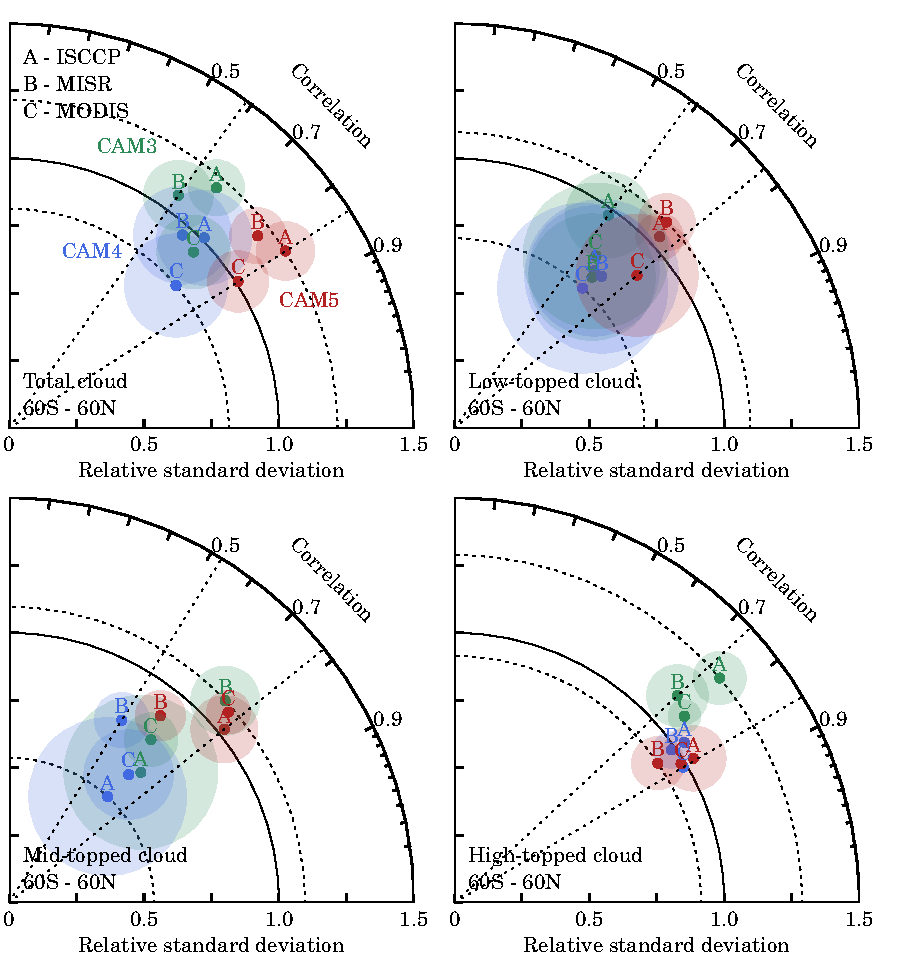
\includegraphics{../graphics/cldtypes_camamip_taylor.pdf}
    \caption[Taylor diagrams comparing total, low-topped, mid-topped, and high-topped ISCCP, MISR, and MODIS-simulated cloud amounts from CAM3, CAM4, and CAM5 AMIP simulations with the corresponding satellite retrievals.]{Taylor diagrams comparing total, low-topped, mid-topped, and high-topped ISCCP, MISR, and MODIS-simulated cloud amounts from CAM3, CAM4, and CAM5 AMIP simulations with the corresponding satellite retrievals. MODIS cloud amounts are taken before clear-sky restoral.}
    \label{cldtypes_camamip_taylor}
\end{figure}

As shown in the previous chapter, CAM3 and AM2 compensate for the underestimation of total and low-topped cloud with a high bias in cloud optical thickness. A principle result of the \cite{kay_et_al_2011} study is the reduction of the cloud optical thickness bias in the CAM5 simulation relative to the CAM4 simulation and to other models documented in the literature \citep[e.g.,][]{zhang_et_al_2005}. This result is demonstrated in Figure \ref{tau_camamip}. Both CAM3 and CAM4 simulations underestimate the amount of optically thin and optically intermediate cloud while overestimating the amount of optically thick cloud. This comparison also shows a large difference between the CAM3 and CAM4 simulations. Both have a similar bias in the distribution of cloudiness toward higher optical thickness, but the CAM4 simulation has a much lower amount of cloud with optical thickness $23.0 < \tau < 60.0$. The increased negative bias in cloud amount in CAM4 relative to CAM3 is primarily due to a reduction in this optically thick cloud.

\begin{figure}
    \centering
    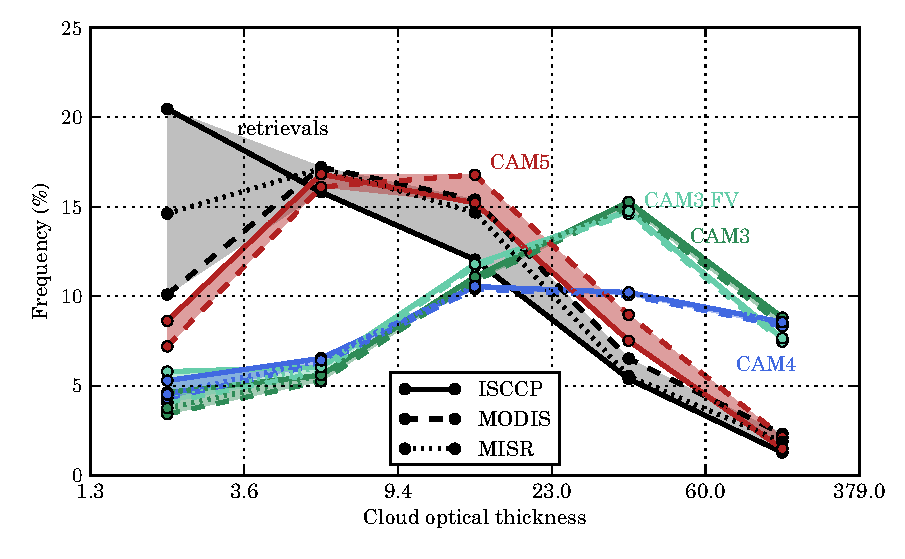
\includegraphics{../graphics/tau_camamip.pdf}
    \caption{Global annual mean histograms of cloudiness with cloud optical thickness from ISCCP, MISR, and MODIS and the corresponding simulator diagnostics from CAM3, CAM4, and CAM5 AMIP simulations.}
    \label{tau_camamip}
\end{figure}
\begin{figure}
    \centering
    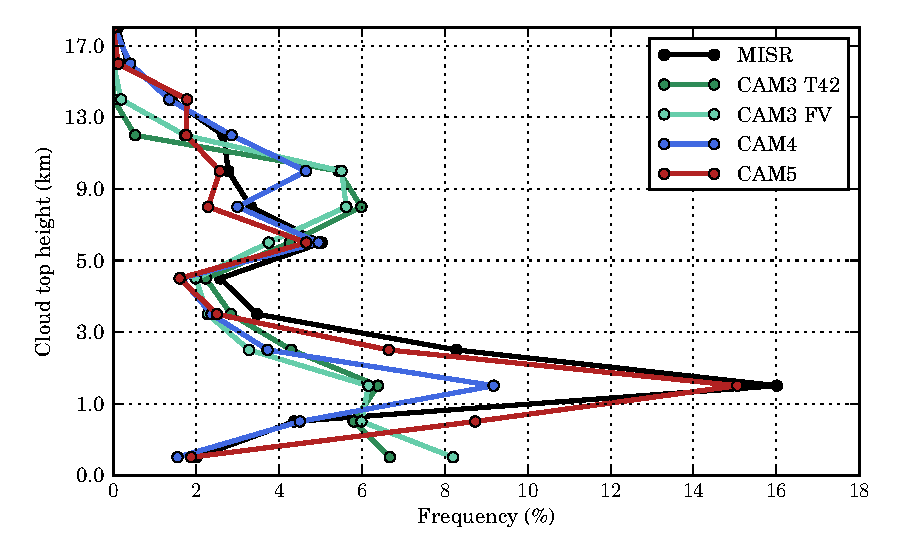
\includegraphics{../graphics/cth_camamip.pdf}
    \caption{Global annual mean histograms of cloudiness with cloud top height from MISR and the MISR simulator diagnostic from CAM3, CAM4, and CAM5 AMIP simulations.}
    \label{cth_camamip}
\end{figure}


Figure \ref{cth_camamip} shows that the distribution of MISR-simulated cloudiness with cloud top height in the CAM5 simulation more closely matches observations than previous versions of the model. A surprising result illustrated by Figure \ref{cth_camamip} is the difference in the distribution of MISR-simulated cloudiness with cloud top height in the CAM4 simulation relative to the two CAM3 simulations, despite the fact that these models use similar subgrid-scale parameterizations. The distributions from the two CAM3 simulations show a large frequency of cloud with cloud tops below $0.5$ km and a sharp decline between $0.5$ km and $1.0$ km, while the distribution from the CAM4 simulation shows an increase in frequency over this entire range. Due to the finite vertical resolution in the models, the histogram binning can exacerbate the impact of differences in the vertical structure on these comparisons. When relatively few model levels coincide with a vertical histogram bin, small changes in the vertical structure of clouds between models could shift a large population of cloud to adjacent histogram bins. Figure \ref{cl_camamip} shows the distribution of the model-diagnosed cloud amount with vertical level (\emph{not} instrument-simulated). This figure demonstrates that CAM3 and CAM4 do in fact simulate different distributions of cloud as seen by the model. It is also important to keep in mind that the diagnosis of MISR-simulated cloudiness depends not only on the model cloud fraction, but on the optical thickness and emissivity on model levels as well, and differences in these quantities may also contribute to differences in the MISR-simulated distributions from CAM3 and CAM4. Nonetheless, Figures \ref{cth_camamip} and \ref{cl_camamip} show that the vertical structure of clouds differs in CAM3 and CAM4. Differences in the distributions of MISR-simulated cloudiness with cloud top height from the CAM3 T42 and CAM3 FV simulations are much smaller than the differences between the distributions from either of the CAM3 simulations and the CAM4 simulation, despite using entirely different dynamical cores. This shows that something beyond a difference in dynamics is responsible for the differences in the distribution of cloudiness with cloud top height between the CAM3 and CAM4 simulations.

\begin{figure}
    \centering
    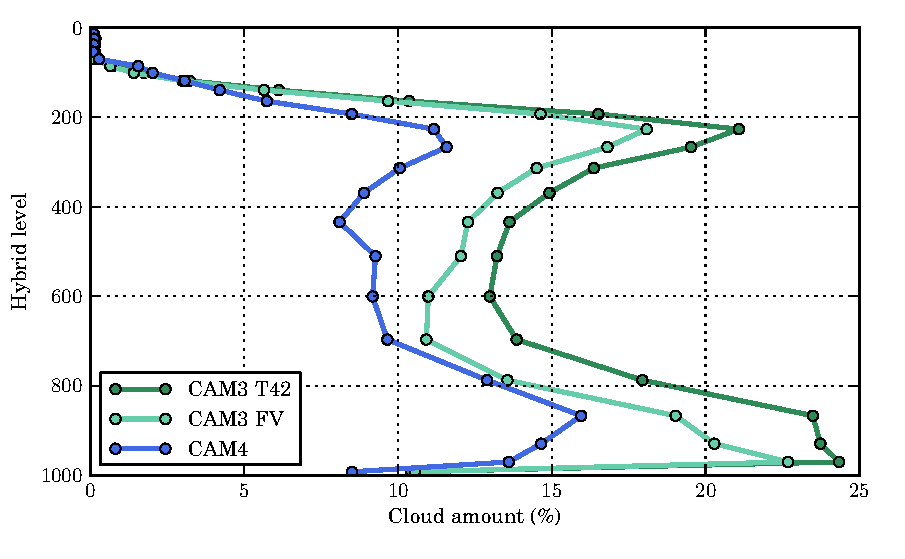
\includegraphics{../graphics/cl_camamip.pdf}
    \caption{Model-diagnosed cloud fraction by model level from CAM3 and CAM4 AMIP simulations.}
    \label{cl_camamip}
\end{figure}

\subsection{Cloudiness in the tropics and subtropics}
Following the approach of the previous chapter, Figure \ref{cldcth_camamip_gpci} shows the distribution of cloudiness with cloud top height along the GPCI Pacific transect \citep{teixeira_et_al_2011}. The far right side of each plot corresponds to the region just off the coast of California. This region is characterized by large-scale subsidence and persistent stratocumulus. Both CAM4 and CAM5 simulations seem to underestimate cloud in the California stratocumulus region (Table \ref{regions}), as evidenced by Figure \ref{jointHist_camamip_CaliforniaStrat_JJA}. Figure \ref{cldcth_camamip_gpci} shows that at least in the CAM5 simulation, a large part of this is likely due to the stratocumulus being concentrated too close to the coast and breaking up into shallow cumulus too quickly. Despite this, the CAM5 simulation does show a larger cloud amount in this region in closer agreement with the observations than the CAM4 simulation. The increase in cloud amount comes primarily from an increase in low-topped optically intermediate cloud, as shown by Figure \ref{jointHist_camamip_CaliforniaStrat_JJA}. This, combined with a decrease relative to the CAM4 simulation of low-topped optically thick cloud brings the distribution of cloudiness with cloud optical thickness in this region in CAM5 closer to observations, as noted by \cite{kay_et_al_2011}, but optically thin cloud is still underestimated in this region.

\begin{figure}
    \centering
    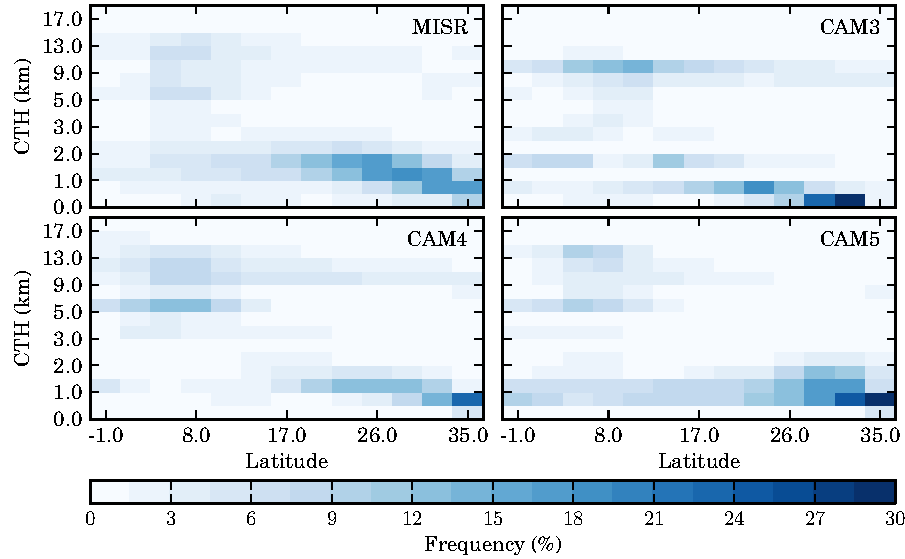
\includegraphics{../graphics/cldcth_camamip_gpci.pdf}
    \caption[Histograms of summertime cloudiness with cloud top height along the GPCI Pacific transect from MISR and the MISR simulator diagnostic from CAM4 and CAM5 AMIP simulations.]{Histograms of summertime (June, July, August) cloudiness with cloud top height along the GPCI Pacific transect from MISR and the MISR simulator diagnostic from CAM4 and CAM5 AMIP simulations.}
    \label{cldcth_camamip_gpci}
\end{figure}

Stratocumulus in the CAM5 simulation seems to transition too early into the cumulus regime, while the CAM4 simulation shows a uniform vertical and geographic distribution of cloudiness from the stratocumulus region to about $20~^\circ\text{N}$, where a sharp transition occurs. This transition in the CAM4 simulation is similar to that seen in the CAM3 simulation. None of the simulations capture the rising of cloud tops in the transition from stratocumulus to trade cumulus.

\begin{figure}
    \centering
    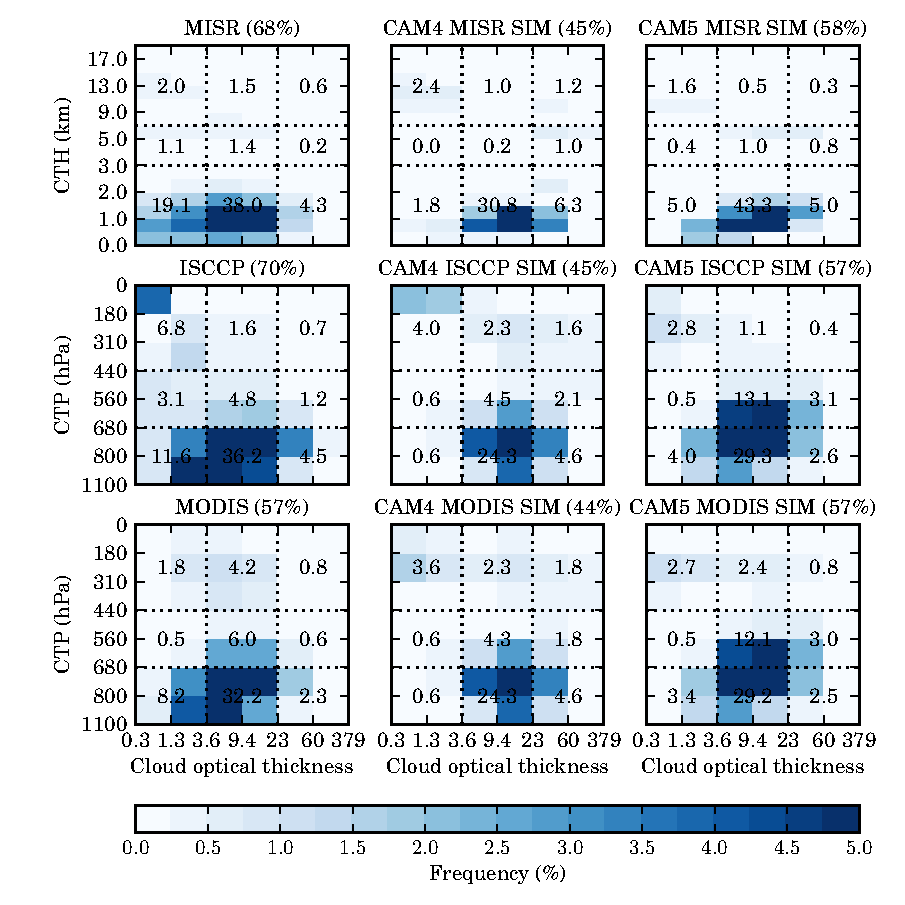
\includegraphics{../graphics/hist2d_camamip_california.pdf}
    \caption[California stratocumulus joint histogram of summertime cloudiness with cloud optical thickness and cloud top height from MISR, ISCCP, and MODIS and the corresponding simulator diagnostics from CAM4 and CAM5 AMIP simulations.]{California stratocumulus (Table \ref{regions}) joint histogram of summertime (June, July, August) cloudiness with cloud optical thickness and cloud top height (or pressure) from MISR, ISCCP, and MODIS and the corresponding simulator diagnostics from CAM4 and CAM5 AMIP simulations.}
    \label{jointHist_camamip_CaliforniaStrat_JJA}
\end{figure}

The far left side of Figure \ref{cldcth_camamip_gpci} corresponds to the deep convective region in the central Pacific in the ITCZ. Both model versions seem to overestimate the amount of high-topped cloud in this region. This bias in high-topped cloud amount results in a large positive bias in the longwave cloud radiative effect in this region in CAM3, CAM4 and, to a lesser extent, in CAM5. This bias does not exist in in the tropical western Pacific region (Figure \ref{jointHist_camamip_TropicalWPacific_JJA}) in either model, although the distribution of cloudiness is biased toward higher optical thickness throughout the vertical in both CAM4 and CAM5 model simulations, similar to that demonstrated in the previous chapter for the CAM3 and AM2 simulations. This bias is reduced in the CAM5 simulation, which brings the distribution closer to observations.

\begin{figure}
    \centering
    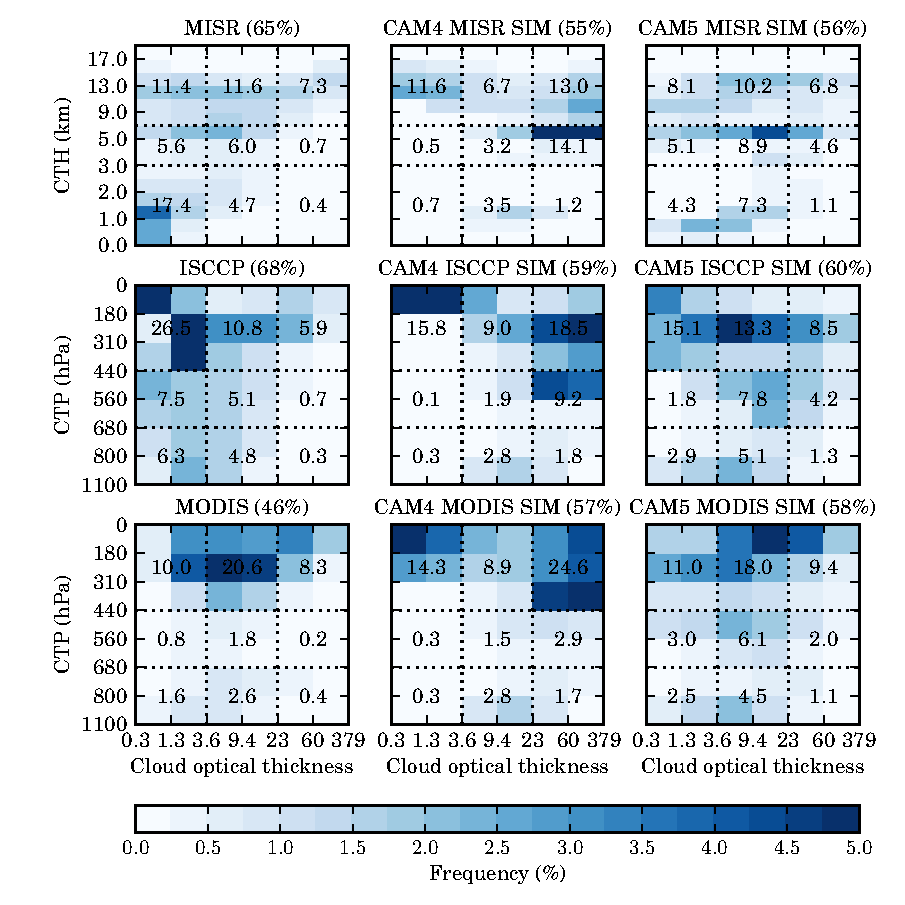
\includegraphics{../graphics/hist2d_camamip_twp.pdf}
    \caption[Tropical western Pacific joint histogram of summertime cloudiness with cloud optical thickness and cloud top height from MISR, ISCCP, and MODIS and the corresponding simulator diagnostics from CAM4 and CAM5 AMIP simulations.]{California stratocumulus (Table \ref{regions}) joint histogram of summertime (June, July, August) cloudiness with cloud optical thickness and cloud top height (or pressure) from MISR, ISCCP, and MODIS and the corresponding simulator diagnostics from CAM4 and CAM5 AMIP simulations.}
    \label{jointHist_camamip_TropicalWPacific_JJA}
\end{figure}

Both CAM4 and CAM5 do simulate the cloud layer associated with the tropical freezing level \citep{johnson_et_al_1999} seen in the MISR observations, although both simulations overestimate the amount of this cloud. This cloud layer is not seen in the CAM3 simulation, so this represents an improvement from CAM3.

\section{Discussion}
Diagnostics using satellite instrument simulators are useful tools in evaluating the representation of clouds in climate models and assessing changes in cloud properties associated with the introduction of new model formulations. The results shown here provide a compliment to those presented in \cite{kay_et_al_2011} by focusing on output from the passive sensor instrument simulators and extending the analysis to assess changes since CAM3.

The use of satellite instrument simulators in this study allows for evaluation of model performance using multiple independent observational datasets quantifying clouds and their radiative properties. Compensating biases in the cloud properties are exposed that may permit reasonable estimates of top of atmosphere energy fluxes with cloud property statistics that differ from reality. In particular, the models studied here have a tendency to compensate for an underestimation of cloud amount with an overestimation of cloud optical thickness. The overestimation of optically thick and the underestimation of optically thin clouds is a common model bias \citep{zhang_et_al_2005}. Changes made in the formulation of CAM5 have reduced the global annual mean bias in simulations with this model.

Total cloudiness is chronically underestimated in all three CAM versions, largely due to underestimation of low and mid-topped cloud. This is especially true for CAM3 and CAM4. The underestimation of mid-topped and, to a lesser extent, low-topped cloud is another common model bias documented in \cite{zhang_et_al_2005}. These biases are greatly reduced in CAM5. \cite{kay_et_al_2011} increase the robustness of this result by adding comparisons with CALIPSO observations.

Despite the improvement in the CAM5 representation of clouds by nearly every measure documented here, large biases remain. Regional biases remain in the cloud properties themselves and in their impact on top of atmosphere radiative fluxes as quantified by the shortwave and longwave cloud radiative effect. Spatial and temporal correlations of these properties between model and observations remain well below correlations between the different observational sets.

Simulation of boundary layer clouds in regions of large-scale subsidence remains troublesome in CAM4 and CAM5. Studies such as that of \cite{bony_and_dufresne_2005} point to the importance of these cloud types to tropical feedbacks. This suggests that efforts to improve the representation of these cloud types in CAM5 will be important.

Despite sharing many physical parameterizations there are substantial differences in the simulation of clouds in CAM3 and CAM4. Experiments substituting the dynamical core in CAM3 suggest that the causes of the changes are rooted elsewhere. It is important to track down the source of these discrepancies as situations such as this provide an opportunity to gain insight into the effect of different changes in the model formulation on the simulation of clouds in climate models. These changes will be invested further in future work.
